\section{Simulation Analysis}
\label{sec:simulation}

\subsection{Simulation - Topic I}
\label{subsec:sim_first}

\begin{table}[H] \centering
  \begin{tabular}{|l|r|}
    \hline    
    {\bf Node/Component} & {\bf Value [A or V]} \\ \hline
    \input{op1_TAB}
  \end{tabular}
  \caption*{XXXXXXXXXXXXXXXXXXXXXXXXXXXXXXXXXXXXXXXXXXXXXXXXXXXXXXXXXXXXXXXXXXXXXX}
 \label{tab:op1}
\end{table}

\paragraph{}
For topic 1 of the simulation analysis section, we can see, in this table, the results of the simulation used to determine the voltages and the currents in all nodes and in all branches, respectively, by simulating the operating point for $t<0$.
%%%%%%%%%%%%%%%%%%%%%%%%%%%%%%%%%%%%%%%%%%%%%%%

\subsection{Simulation - Topic II}
\label{subsec:sim_second}

\begin{table}[H] \centering
  \begin{tabular}{|l|r|}
    \hline    
    {\bf Node/Component} & {\bf Value [A or V]} \\ \hline
    \input{op2_TAB}
  \end{tabular}
  \caption*{XXXXXXXXXXXXXXXXXXXXXXXXXXXXXXXXXXXXXXXXXXXXXXXXXXXXXXXXXXXXXXXXXXXXXX}
 \label{tab:op1}
\end{table}

\paragraph{}
For topic 2, by simulating the operating point for $vs(0)=0$, and replacing the capacitor with a voltage source $Vx = V(6)-V(8)$, where V(6) and V(8) are the voltages in nodes 6 and 8 as obtained in topic 1, we obtain the results printed in tabel above. We do this step in order to use Thevenin´s Theorem to simplify this complex circuit, turning it into a more simple equivalent circuit consisting of a resistance in series with a source voltage.
%%%%%%%%%%%%%%%%%%%%%%%%%%%%%%%%%%%%%%%%%%%%%%%

\subsection{Simulation - Topic III}
\label{subsec:sim_third}

\begin{figure}[H] \centering
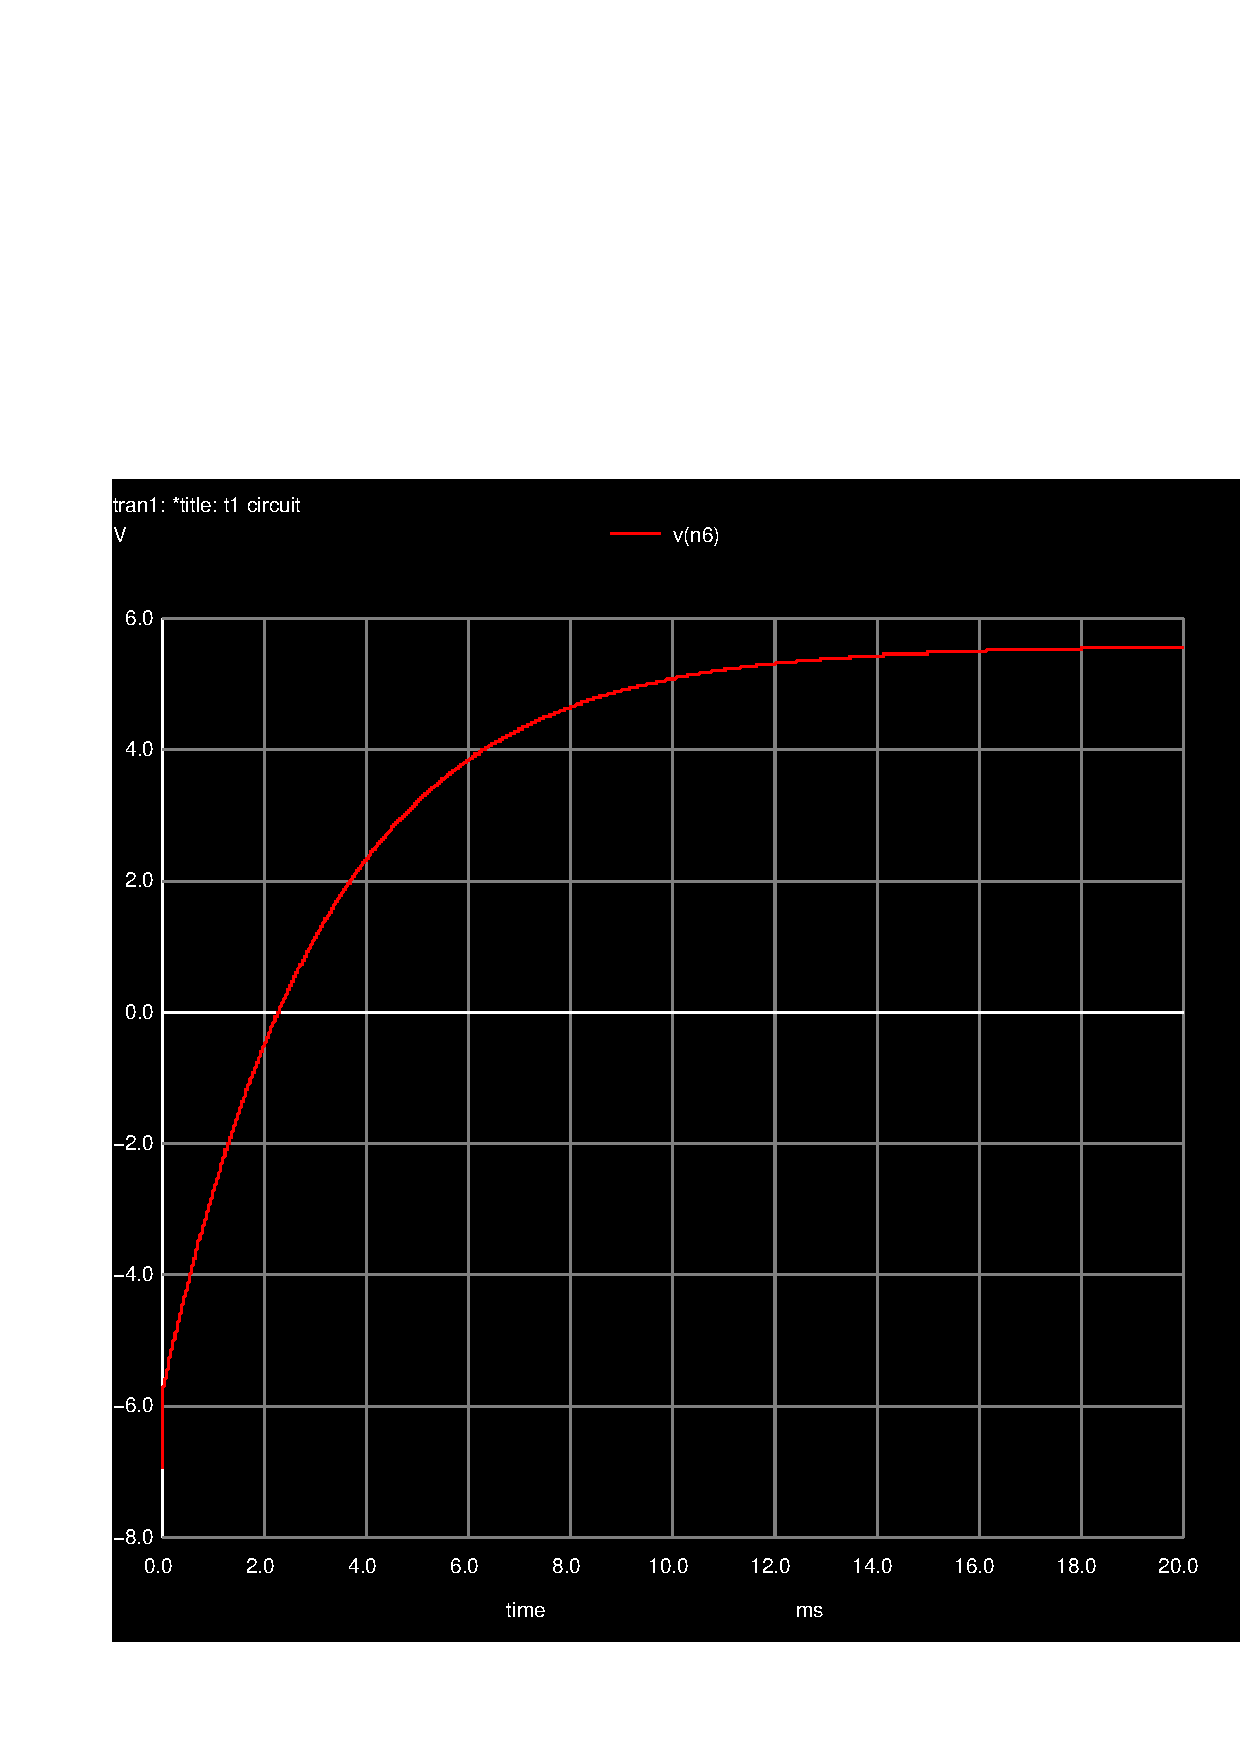
\includegraphics[width=0.4\textwidth]{trans1.pdf}
\caption{Natural response of the circuit}
\label{fig:natural}
\end{figure}

\paragraph{}
For topic 3, by using the boundary conditions V(6) and V(8) obtained in topic 2, and by using Ngspice’s transient analysis mode to get v6(t) in the interval [0, 20] ms, we can simulate the natural response of the circuit and plot the results, as presented in the figure above.

%%%%%%%%%%%%%%%%%%%%%%%%%%%%%%%%%%%%%%%%%%%%%%%

\subsection{Simulation - Topic IV}
\label{subsec:sim_fourth}

\begin{figure}[H] \centering
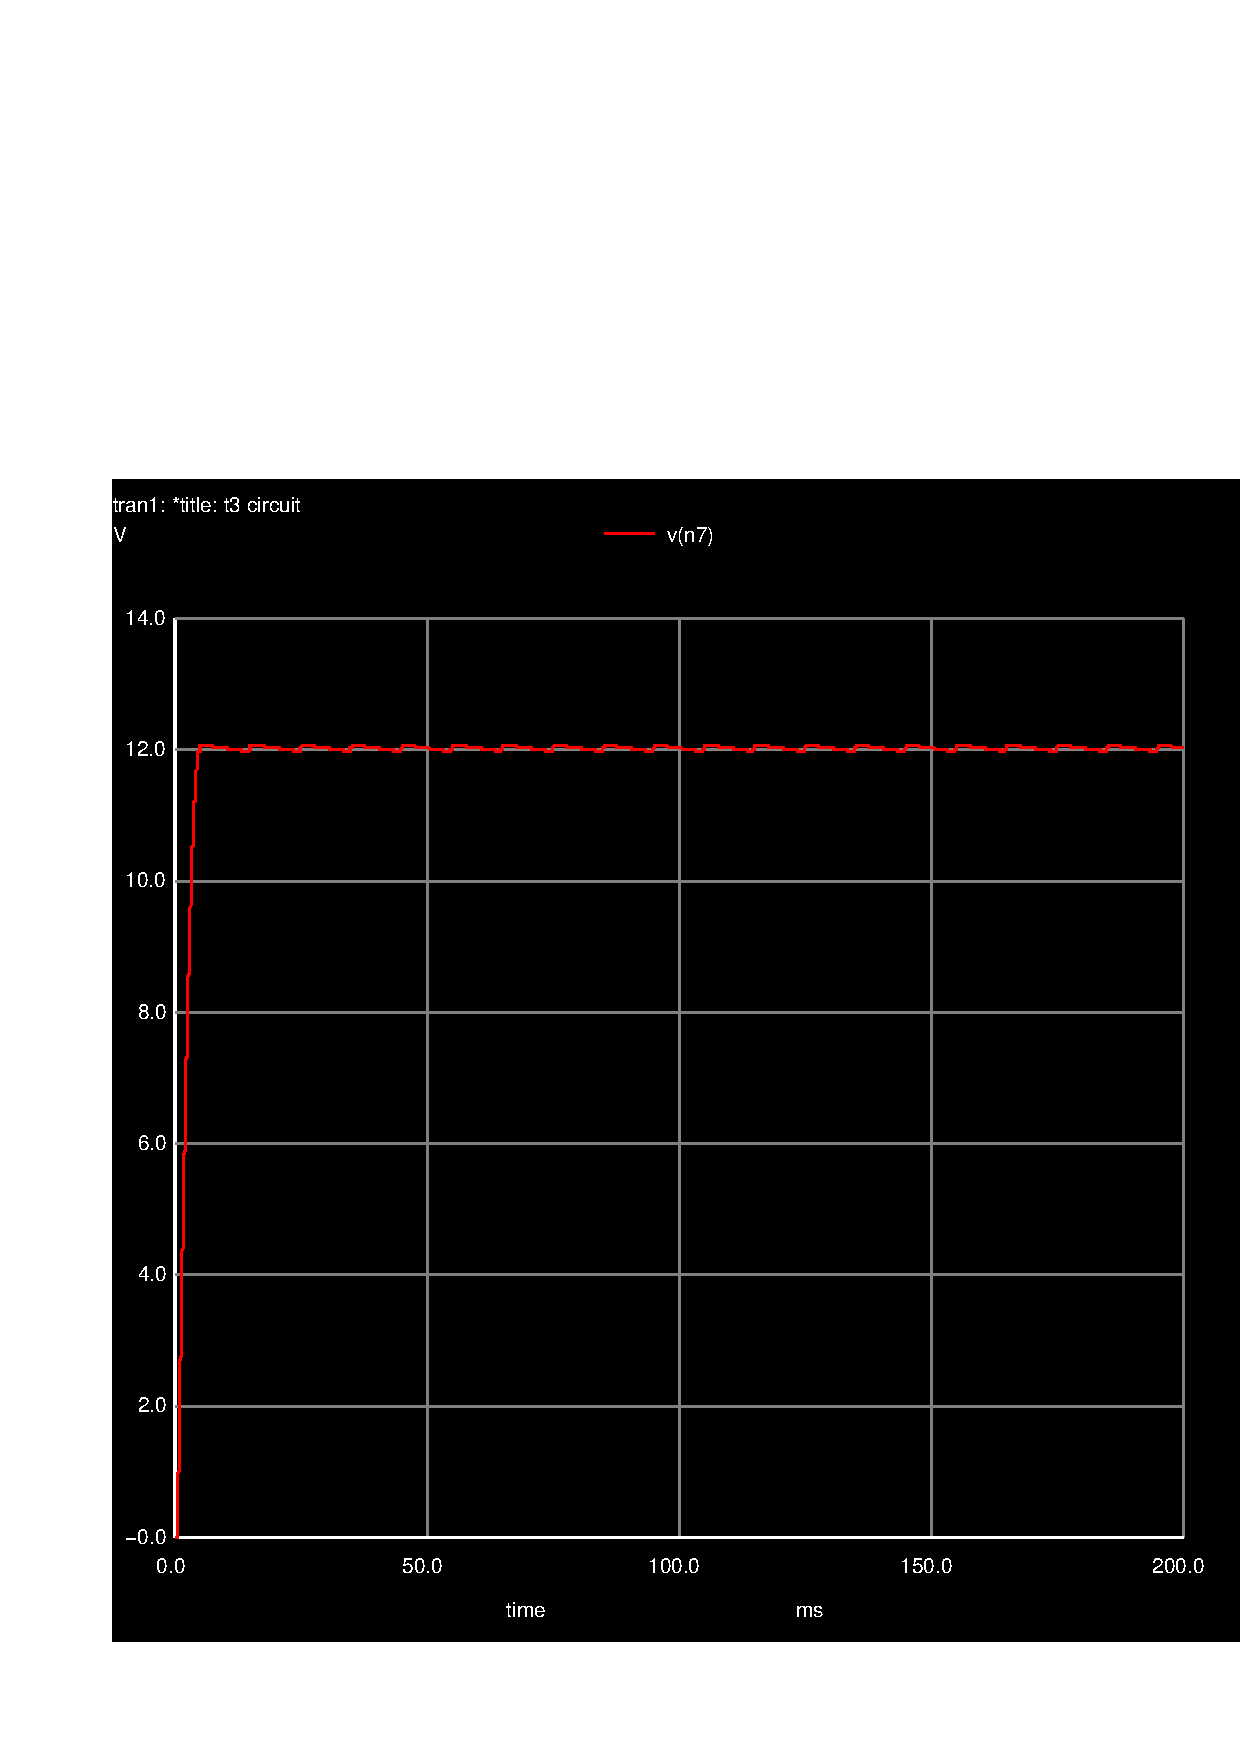
\includegraphics[width=0.4\textwidth]{trans2.pdf}
\caption{Total response of the circuit}
\label{fig:total}
\end{figure}

\paragraph{}
Regarding topic 4, the above figure is ploted by simulating the total response on node 6, that is, the natural and the forced solutions, by repeating the step presented in topic 3 with $v_s(t) = V_s u(-t) + sin(2 \pi ft) u(t)$ and frequency equal to 1 $KH_z$. 

%%%%%%%%%%%%%%%%%%%%%%%%%%%%%%%%%%%%%%%%%%%%%%%%%%

\subsection{Simulation - Topic V}
\label{subsec:sim_fifth}

\begin{figure}[H] \centering
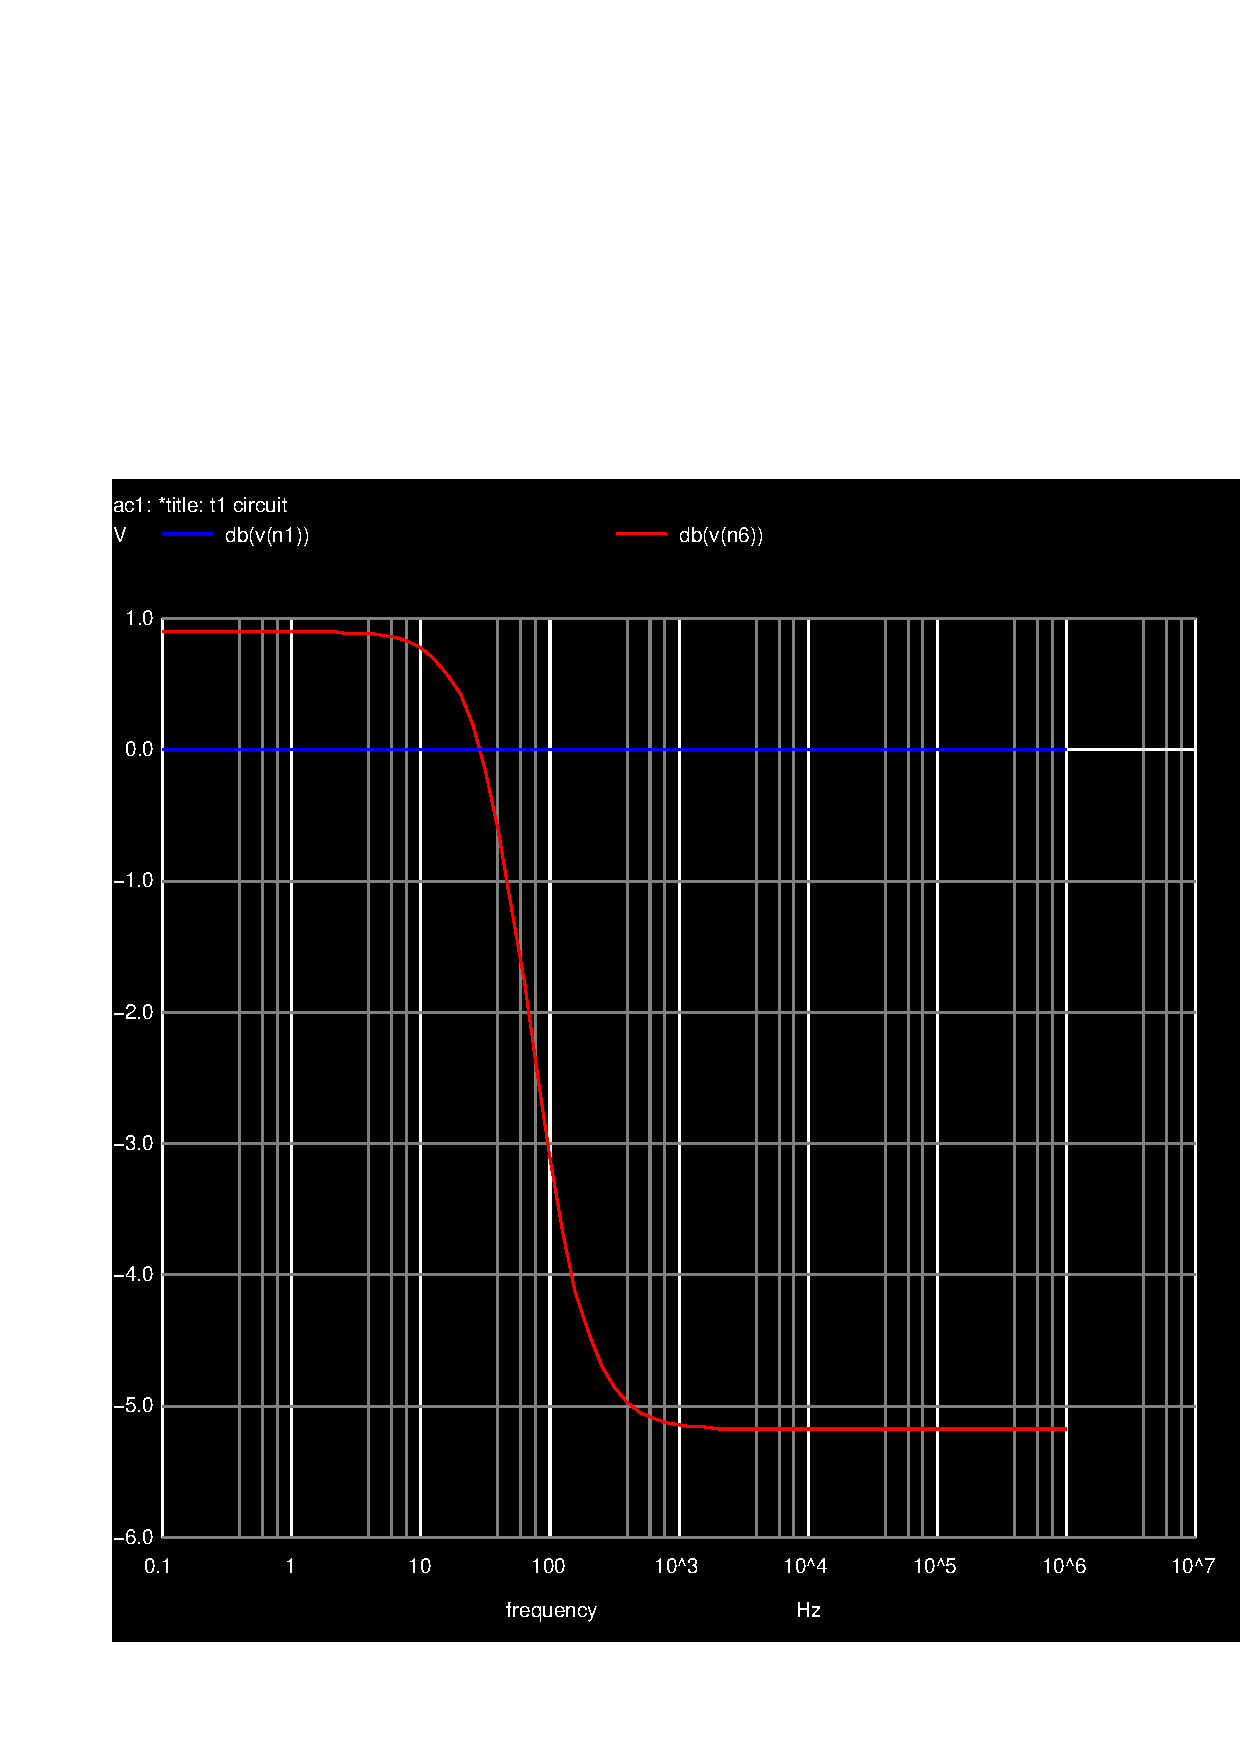
\includegraphics[width=0.4\textwidth]{acm.pdf}
\caption{LALALAALALALALALALAL.}
\label{fig:LALALAAL}
\end{figure}


\begin{figure}[H] \centering
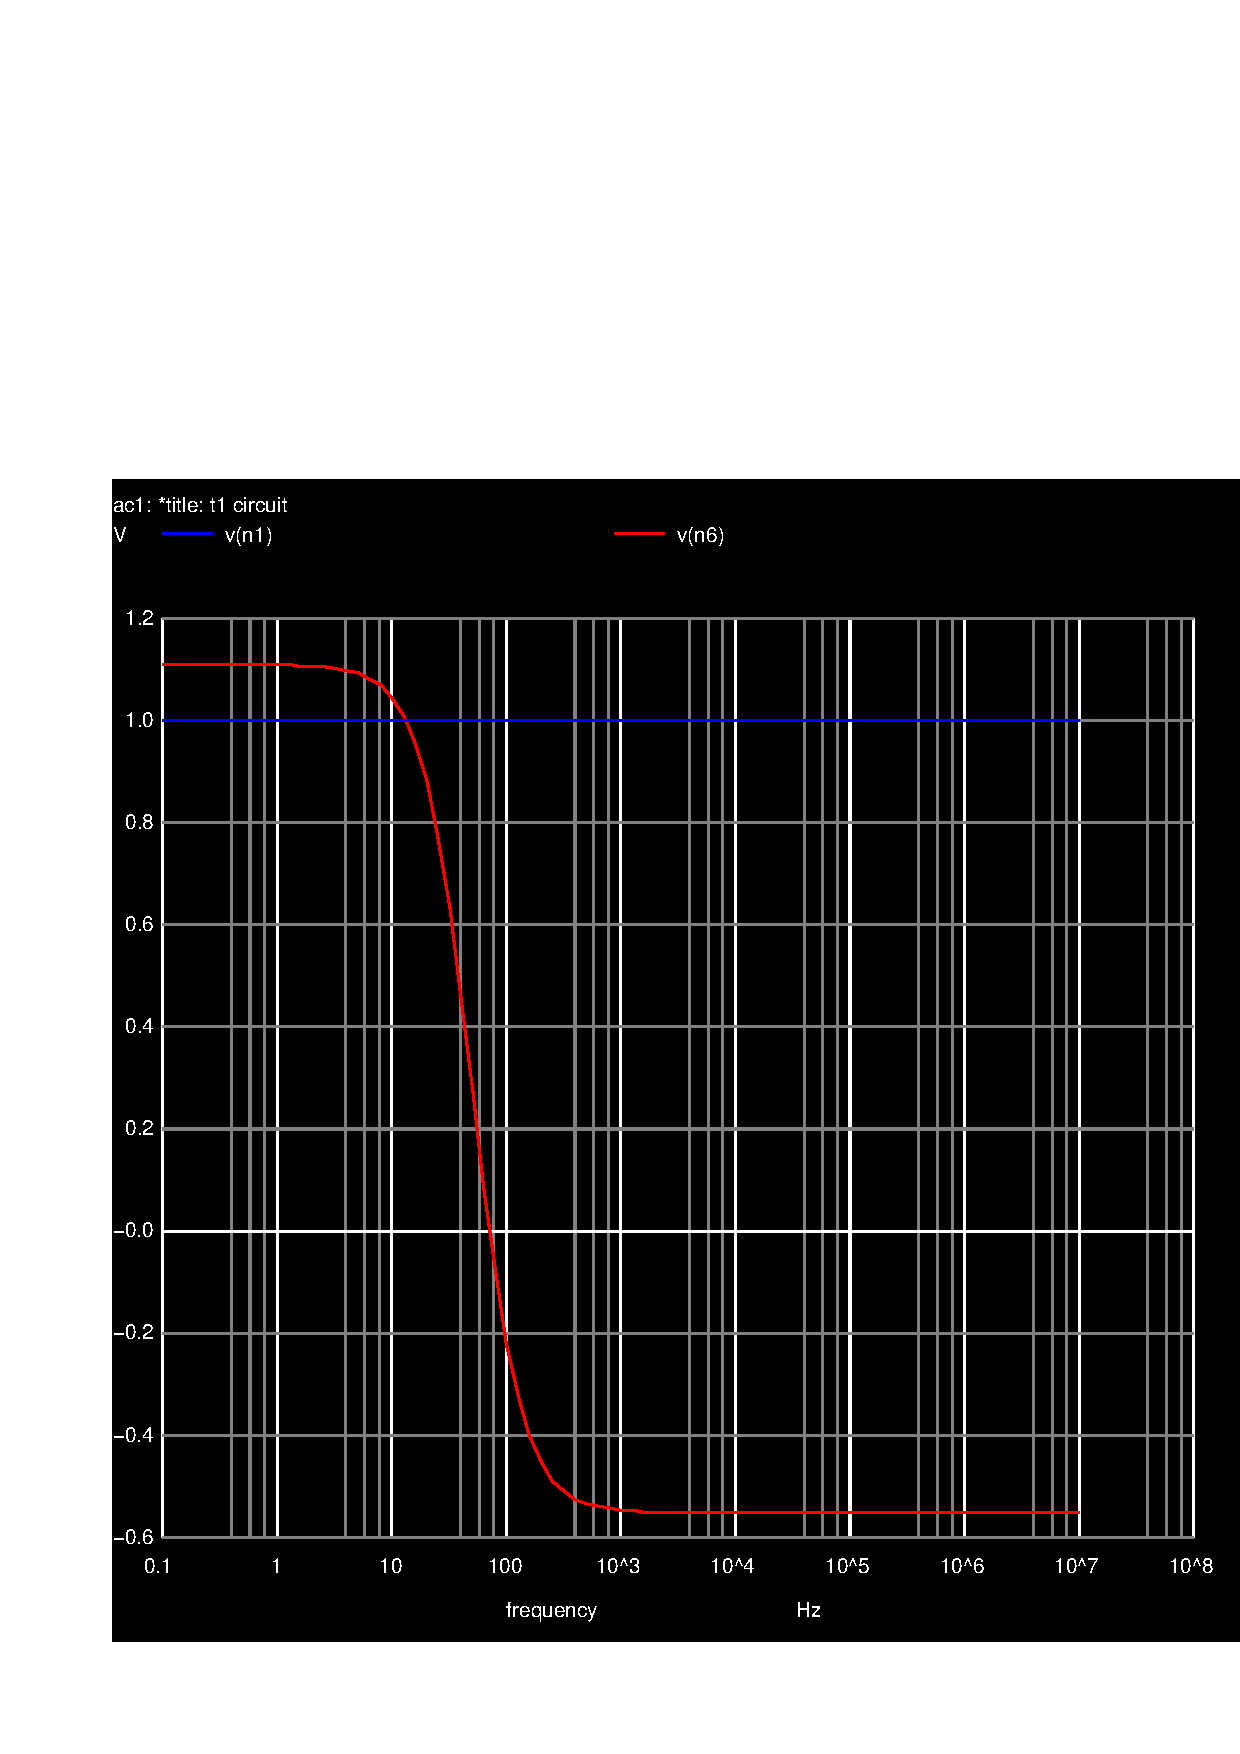
\includegraphics[width=0.4\textwidth]{acp.pdf}
\caption{LALALAALALALALALALAL.}
\label{fig:LALALAAL}
\end{figure}


\pagebreak
